% Options for packages loaded elsewhere
\PassOptionsToPackage{unicode}{hyperref}
\PassOptionsToPackage{hyphens}{url}
%
\documentclass[
  12pt,
]{article}
\usepackage{amsmath,amssymb}
\usepackage{lmodern}
\usepackage{ifxetex,ifluatex}
\ifnum 0\ifxetex 1\fi\ifluatex 1\fi=0 % if pdftex
  \usepackage[T1]{fontenc}
  \usepackage[utf8]{inputenc}
  \usepackage{textcomp} % provide euro and other symbols
\else % if luatex or xetex
  \usepackage{unicode-math}
  \defaultfontfeatures{Scale=MatchLowercase}
  \defaultfontfeatures[\rmfamily]{Ligatures=TeX,Scale=1}
\fi
% Use upquote if available, for straight quotes in verbatim environments
\IfFileExists{upquote.sty}{\usepackage{upquote}}{}
\IfFileExists{microtype.sty}{% use microtype if available
  \usepackage[]{microtype}
  \UseMicrotypeSet[protrusion]{basicmath} % disable protrusion for tt fonts
}{}
\makeatletter
\@ifundefined{KOMAClassName}{% if non-KOMA class
  \IfFileExists{parskip.sty}{%
    \usepackage{parskip}
  }{% else
    \setlength{\parindent}{0pt}
    \setlength{\parskip}{6pt plus 2pt minus 1pt}}
}{% if KOMA class
  \KOMAoptions{parskip=half}}
\makeatother
\usepackage{xcolor}
\IfFileExists{xurl.sty}{\usepackage{xurl}}{} % add URL line breaks if available
\IfFileExists{bookmark.sty}{\usepackage{bookmark}}{\usepackage{hyperref}}
\hypersetup{
  pdftitle={Methodological details of the norming and production studies},
  hidelinks,
  pdfcreator={LaTeX via pandoc}}
\urlstyle{same} % disable monospaced font for URLs
\usepackage[margin=1in]{geometry}
\usepackage{longtable,booktabs,array}
\usepackage{calc} % for calculating minipage widths
% Correct order of tables after \paragraph or \subparagraph
\usepackage{etoolbox}
\makeatletter
\patchcmd\longtable{\par}{\if@noskipsec\mbox{}\fi\par}{}{}
\makeatother
% Allow footnotes in longtable head/foot
\IfFileExists{footnotehyper.sty}{\usepackage{footnotehyper}}{\usepackage{footnote}}
\makesavenoteenv{longtable}
\usepackage{graphicx}
\makeatletter
\def\maxwidth{\ifdim\Gin@nat@width>\linewidth\linewidth\else\Gin@nat@width\fi}
\def\maxheight{\ifdim\Gin@nat@height>\textheight\textheight\else\Gin@nat@height\fi}
\makeatother
% Scale images if necessary, so that they will not overflow the page
% margins by default, and it is still possible to overwrite the defaults
% using explicit options in \includegraphics[width, height, ...]{}
\setkeys{Gin}{width=\maxwidth,height=\maxheight,keepaspectratio}
% Set default figure placement to htbp
\makeatletter
\def\fps@figure{htbp}
\makeatother
\setlength{\emergencystretch}{3em} % prevent overfull lines
\providecommand{\tightlist}{%
  \setlength{\itemsep}{0pt}\setlength{\parskip}{0pt}}
\setcounter{secnumdepth}{5}
\renewcommand{\familydefault}{\sfdefault}
\usepackage{expex}
\lingset{everygla=,everyglpreamble=\it}
\usepackage[export]{adjustbox}
\ifluatex
  \usepackage{selnolig}  % disable illegal ligatures
\fi

\title{Methodological details of the norming and production studies}
\author{}
\date{\vspace{-2.5em}9/17/2020}

\begin{document}
\maketitle

{
\setcounter{tocdepth}{2}
\tableofcontents
}
\hypertarget{overview}{%
\section{Overview}\label{overview}}

This document describes the methodological details of the norming study and the production study that generated the data your team will analyze for the \emph{Many Speech Analyses} project.

The norming study was run to obtain ratings on the typicality of color/object combinations used to create the experimental categories manipulated in the production study.
The production study then investigated whether speakers modify speech to signal the (a)typicality of the color/object combinations.
Concretely, we asked whether the acoustic profile of an utterance with an atypical referent like \emph{blue banana} is different from one with a typical referent such as \emph{yellow banana}.

\hypertarget{norming-study}{%
\section{Norming study}\label{norming-study}}

Here we specify in detail the selection of the stimuli used in the production study.

\hypertarget{selection-of-stimuli-superset}{%
\subsection{Selection of stimuli superset}\label{selection-of-stimuli-superset}}

The selection of stimuli was informed by a norming study for which twenty fruits or vegetables (henceforth: FOODs) and four other referents (henceforth: NON-FOODs) were chosen.
Selection criteria were mainly informed by visual discriminability and phonemic composition, such that nouns denoting objects were supposed to contain as few voiceless segments as possible.

For each of the FOODs and NON-FOODs, we created colored versions by image manipulation using \href{http://www.gimp.org}{Gimp}.
Images of all individual objects were collected from internet databases containing copyright-free high-resolution images (e.g.~\href{https://pixabay.com}{Pixabay}).
During the manipulation process, the background of the pictures was replaced with a white background.
In order to change the color of the objects, a layer in the respective color was created and overlaid on top of the original image using \texttt{Color} as the layer mode.
The hexadecimal color codes for the colors that we used are listed below:

\begin{itemize}
\tightlist
\item
  Blue: \#29429f
\item
  Green: \#3f8535
\item
  Red: \#9d1c1c
\item
  Purple: \#6d1b79
\item
  Brown: \#2a1d11
\item
  Yellow: \#e3c917
\item
  Orange: \#ff8400
\item
  Orange (potatoes): \#ff6600
\item
  Black: \#000
\item
  Grey: \#fff
\end{itemize}

All pictures with natural and manipulated colors are available here: \url{https://osf.io/rdtx5/}.

The colors for the twenty FOODs were subjectively selected to reflect a range of compatibilities with the respective objects, e.g.~a typical banana is yellow; a less typical banana could be brown (too ripe) or green (not yet ripe); and an atypical banana could be blue.
Every FOOD was presented in four of nine manipulated colors alongside its original image.
The four NON-FOODs were subjectively selected to represent color agnostic objects which can and do come in a variety of colors.
All objects were chosen such that their respective German nouns were either feminine singular (e.g.~\emph{die Banana} `the banana') or plural (e.g.~\emph{die Trauben} `the grapes').

We used the following FOODs: apricot, avocado, banana, beans, carrot, cherry, cucumber, eggplant, grapes, lemon, mandarine, pear, pepper, pineapple, potatoes, strawberry, tomato, walnut, zucchini.

We used the following NON-FOODs: clothespin, paper clip, socks, sunglasses.

\hypertarget{participants-and-procedures}{%
\subsection{Participants and procedures}\label{participants-and-procedures}}

A hundred German native speakers participated in a norming study using the crowd sourcing platform \href{https://www.prolific.ac}{Prolific}.
We presented all objects in different colors to our participants.
FOODs came in 5 colors per object, NON-FOODs came in all nine colors.
Participants were instructed to rate how typical they thought the color for each object was, using a smooth slider ranging from 1 to 100 (see javascript for the experimental design here: \url{https://github.com/stelaseldano/colour-typicality-norming}).
The results of the norming study can be retrieved here: \url{https://osf.io/znpg5/}.

\hypertarget{selection-of-experimental-stimuli-for-the-production-study}{%
\subsection{Selection of experimental stimuli for the production study}\label{selection-of-experimental-stimuli-for-the-production-study}}

The typicality ratings were subsequently used to select appropriate stimuli for the production study according to the following procedure:

First, we chose five colors from the norming data set: yellow, green, red, orange, and brown.
Those were the most frequent colors in the superset and their norming results varied strongly as a function of the object.

Second, we sorted the FOODs according to their typicality ratings and binned them into typical, medium, and atypical.
Typical FOODs were defined by norming ratings above 90.
Atypical FOODs were defined by norming ratings below 25.
Medium typical FOODs were defined by norming ratings in between 25 and 90.
For each color and typicality, we selected one FOOD object.
Each cell was occupied by a different FOOD.

For the noun focus condition (NF) this selection procedure resulted in 15 target FOODs (5 colors x 3 typicality categories):

\begin{itemize}
\tightlist
\item
  Atypical:

  \begin{itemize}
  \tightlist
  \item
    Yellow cherry (\emph{Gelbe Kirsche}).
  \item
    Green carrot (\emph{Grüne Möhre}).
  \item
    Red cucumber (\emph{Rote Gurke}).
  \item
    Orange grapes (\emph{Oangene Trauben}).
  \item
    Brown pepper (\emph{Braune Paprika}).
  \end{itemize}
\item
  Medium:

  \begin{itemize}
  \tightlist
  \item
    Yellow peas (\emph{Gelbe Erbsen}).
  \item
    Green tomato (\emph{Grüne Tomate}).
  \item
    Red apricot (\emph{Rote Aprikose}).
  \item
    Orange potatoes (\emph{Orangene Kartoffeln}).
  \item
    Brown banana (\emph{Braune Banane}).
  \end{itemize}
\item
  Typical:

  \begin{itemize}
  \tightlist
  \item
    Yellow lemon (\emph{Gelbe Zitrone}).
  \item
    Green green beans (\emph{Grüne Bohnen}).
  \item
    Red strawberry (\emph{Rote Erdbeere}).
  \item
    Orange mandarine (\emph{Orangene Mandarine}).
  \item
    Brown walnut (\emph{Braune Walnuss}).
  \end{itemize}
\end{itemize}

The set of 15 competitors from the NON-FOOD subset was selected to ensure that there are as many distinct competitors for each color as there are target objects.
The set consisted of the following objects:

\begin{itemize}
\tightlist
\item
  Yellow sunglasses (\emph{Gelbe Sonnenbrille}).
\item
  Yellow socks (\emph{Gelbe Socken}).
\item
  Yellow clothes peg (\emph{Gelbe Wäscheklammer}).
\item
  Green sunglasses (\emph{Grüne Sonnenbrille}).
\item
  Green socks (\emph{Grüne Socken}).
\item
  Green Paper clip (\emph{Grüne Büroklammer}).
\item
  Red socks (\emph{Rote Socken}).
\item
  Red paper clip (\emph{Rote Büroklammer}).
\item
  Red clothes peg (\emph{Rote Wäscheklammer}).
\item
  Orange socks (\emph{Orangene Socken}).
\item
  Orange paper clip (\emph{Orangene Büroklammer})
\item
  Orange clothes peg (\emph{Orangene Wäscheklammer}).
\item
  Brown sunglasses (\emph{Braune Sonnenbrille}).
\item
  Brown paper clip (\emph{Braune Büroklammer}).
\item
  Brown clothes peg (\emph{Braune Wäscheklammer}).
\end{itemize}

For the Adjective and Adjective/Noun conditions (AF + ANF), we distributed FOODs and NON-FOODs to fulfill the following constraints: (a) each target FOOD appeared 3 times and (b) each color appeared as a target color 14 times.

For all three focus conditions, a subset of distractors was selected from the initial superset.
The distractors were either FOODS that were neither used as targets nor as competitors (avocado, egg plant, pear, zucchini) or NON-FOODs.
Within each given trial, the distractors did not share color nor object identity with neither the target nor the competitor.

Overall, the sets of target, competitors and distractors were combined such that all five colors occurred equally often throughout the experiment (i.e.~28 times).

\hypertarget{production-study}{%
\section{Production study}\label{production-study}}

\hypertarget{participants}{%
\subsection{Participants}\label{participants}}

Thirty native German speakers participated in this study.
All participants grew up in a monolingual environment and were recruited from the population living in the broad Cologne area with normal or corrected-to-normal vision and normal hearing.
Participants were paid for their participation.

\hypertarget{procedure}{%
\subsection{Procedure}\label{procedure}}

In this production study, participants interacted with the experimenter in German.
Participants were seated in front of a computer screen.
The experimenter sat at the opposite side of the table in front of another computer screen.
The participants and the experimenter could not see each other nor each others' screens.
The participants had to verbally instruct the experimenter to select a specified target object out of four visually presented objects.
The non-target objects differed from the target with respect to their color, their identity, or both.
Objects were referred to using noun phrases that consist of a modifier denoting color and a modified object (e.g.~\emph{Gelbe Zitrone} `yellow lemon', \emph{Rote Gurke} `red cucumber', \emph{Rote Socken} `red socks').
These color-object combinations differed with respect to their typicality.
The color-object combinations were either typical (e.g.~\emph{Orangene Mandarine} `orange mandarin'), medium typical (e.g.~\emph{Grüne Tomate} `green tomato'), or atypical (e.g.~\emph{Gelbe Kirsche} `yellow cherry').
Figure \ref{fig:image0} illustrates combination typicality for a banana, a tomato, and an apricot.

\begin{figure}[tbp]

{\centering 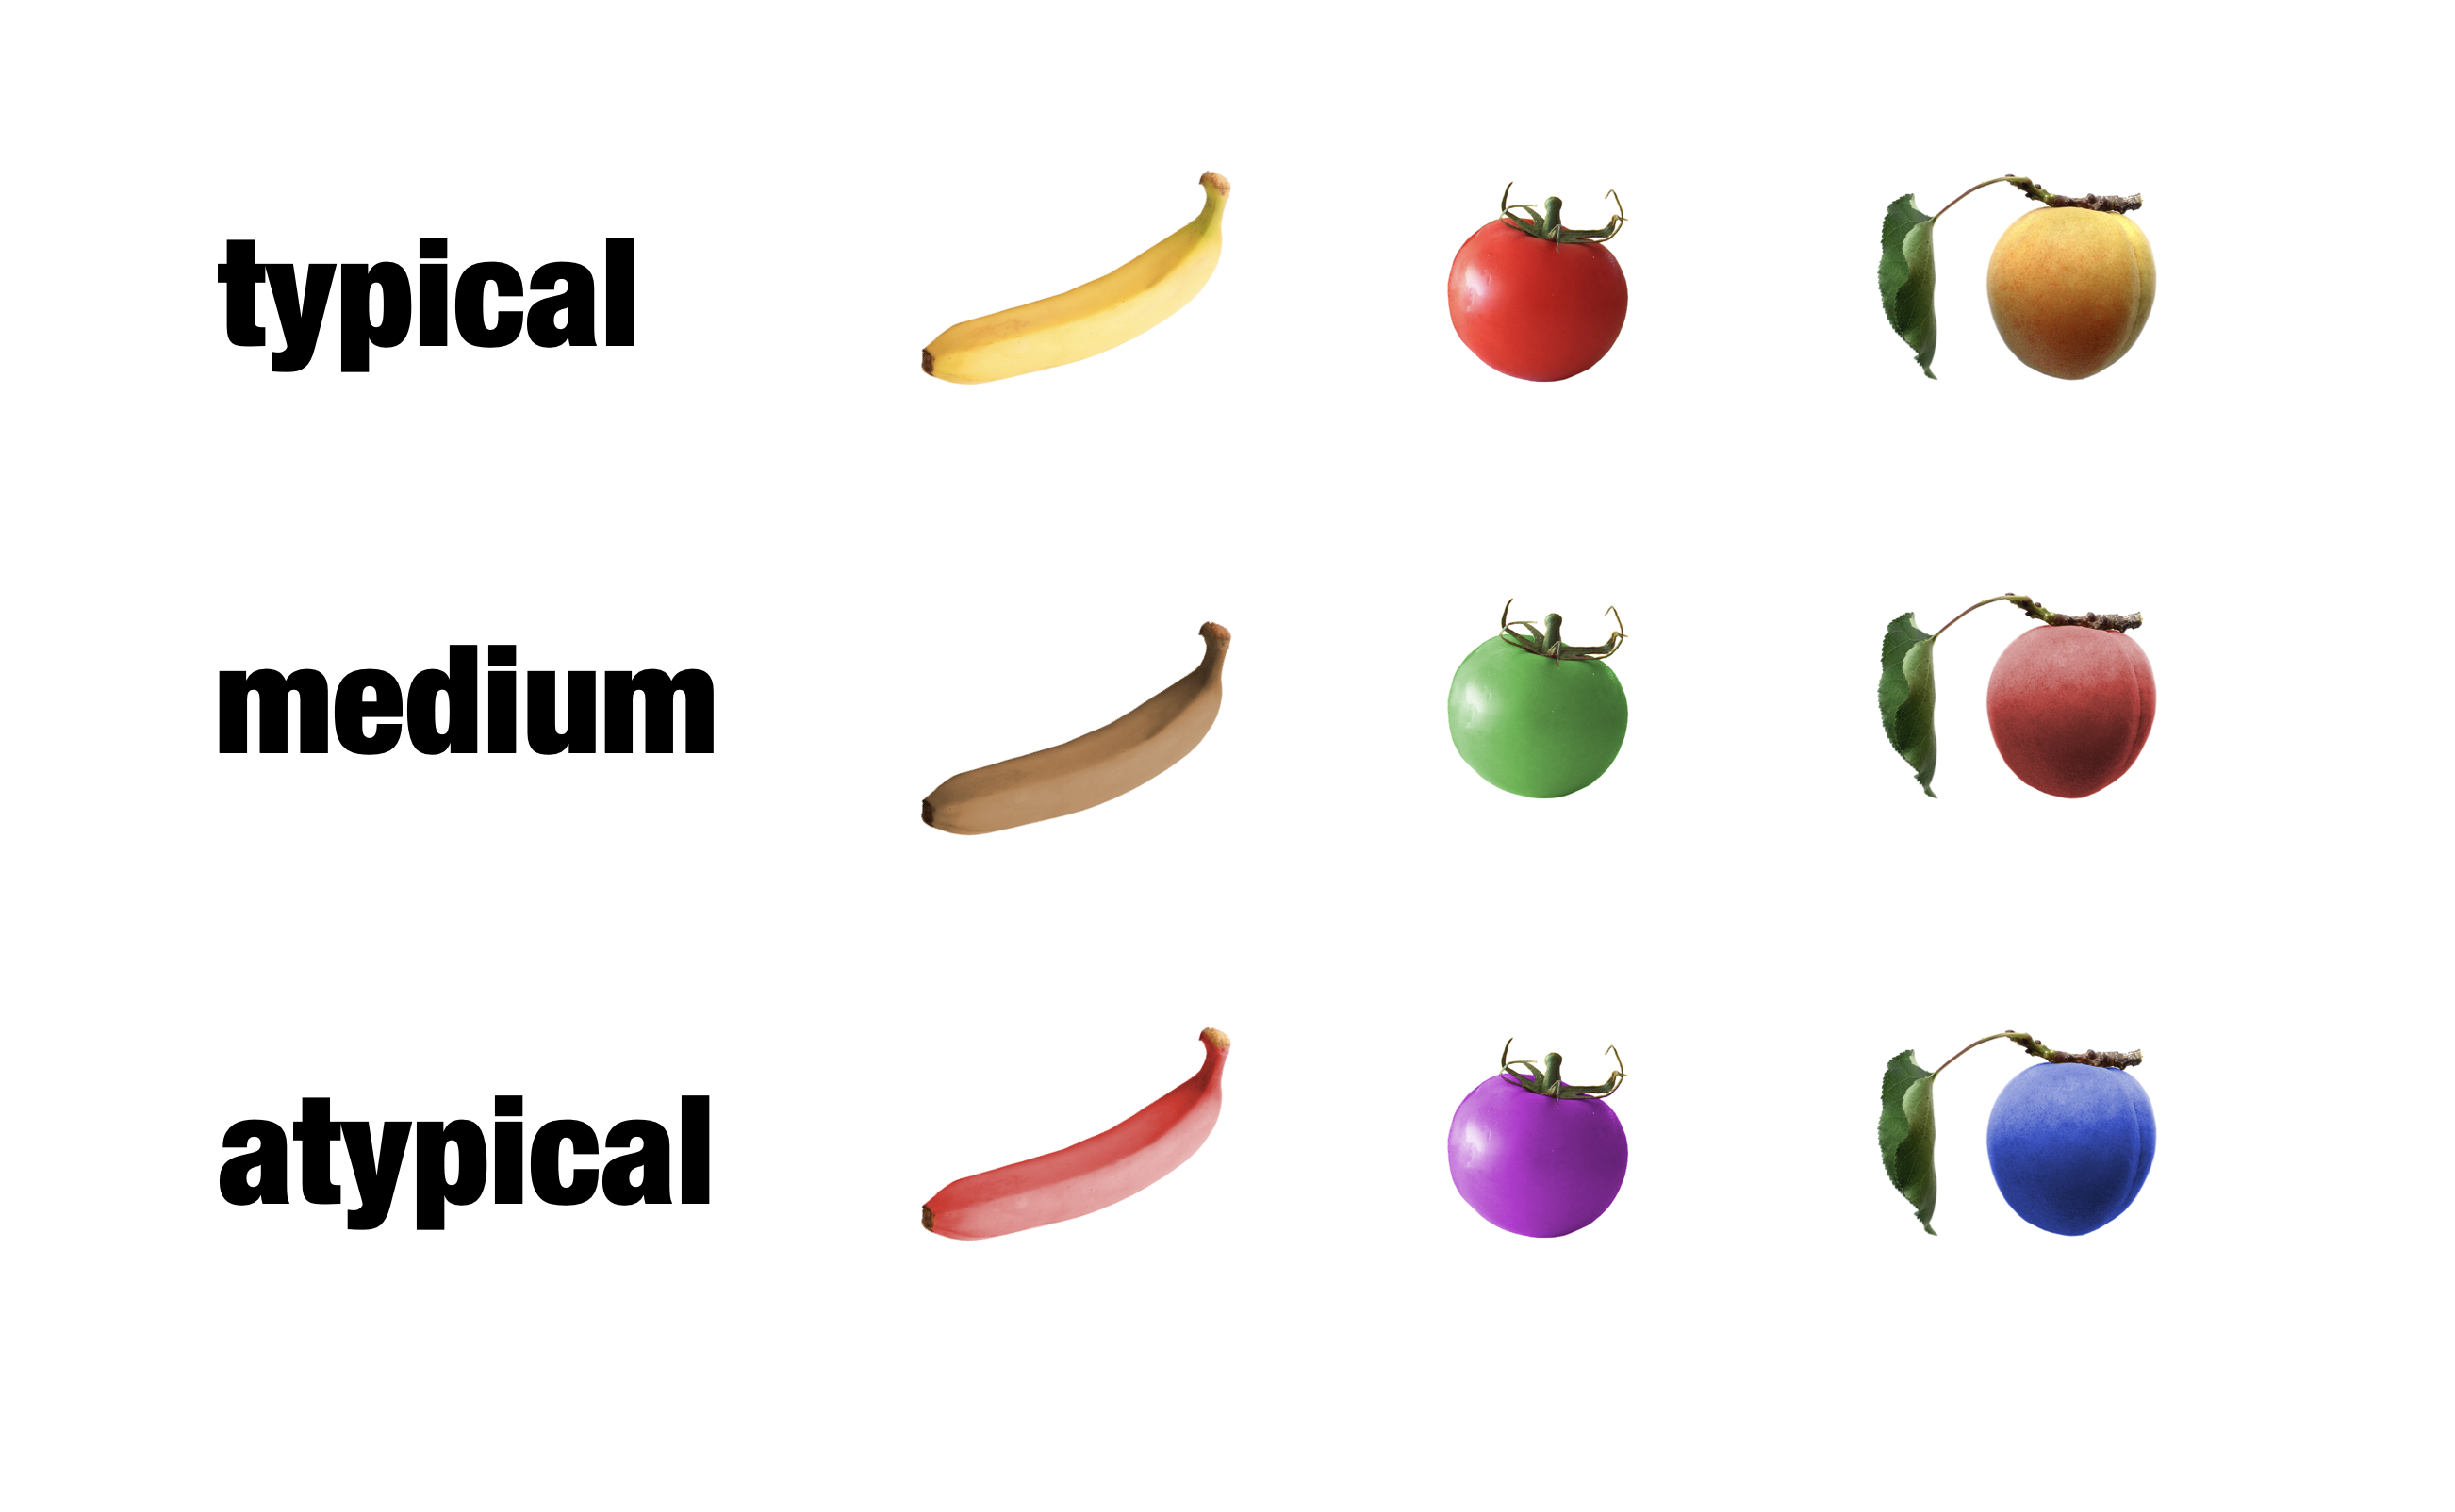
\includegraphics[width=0.6\linewidth]{/Users/ste/repos/many_analyses/figs/typicality_examples} 

}

\caption{Three examples for typical, medium typical and atypical combinations of colour and object.}\label{fig:image0}
\end{figure}

The experiment consisted of two phases: a familiarization phase and a test phase.

In a familiarization phase, participants saw the picture of one object per trial.
In order to advance to the next trial, participants had to read out loud the corresponding color-object combination.
During this phase, participants had to name all atypical color-object targets that we used in the test phase of the experiment alongside their typical counterparts.
For example, one of the experimental targets was a red banana (atypical).
The participants were presented with the picture of both a red banana (atypical) and a yellow banana (typical).
This familiarization phase was included in order to ensure that participants could relate typical and atypical color-object combinations to each other.

After the familiarization phase, the participants entered the test phase.
On each trial in the test phase, the subjects first saw four colored objects in the top left, top right, bottom left, and bottom right of the screen, respectively.
One of the object served as the target; another served as the competitor; and the remaining two served as unrelated distractors.
The position of the visual stimuli was randomized for each trial and each participant (see Appendix \ref{random}).
In the center of the screen, a black cube was displayed, which could be moved by the experimenter.
The participants were asked to instruct the experimenter to move the cube on top of one of the four depicted object.

\begin{figure}[tbp]

{\centering 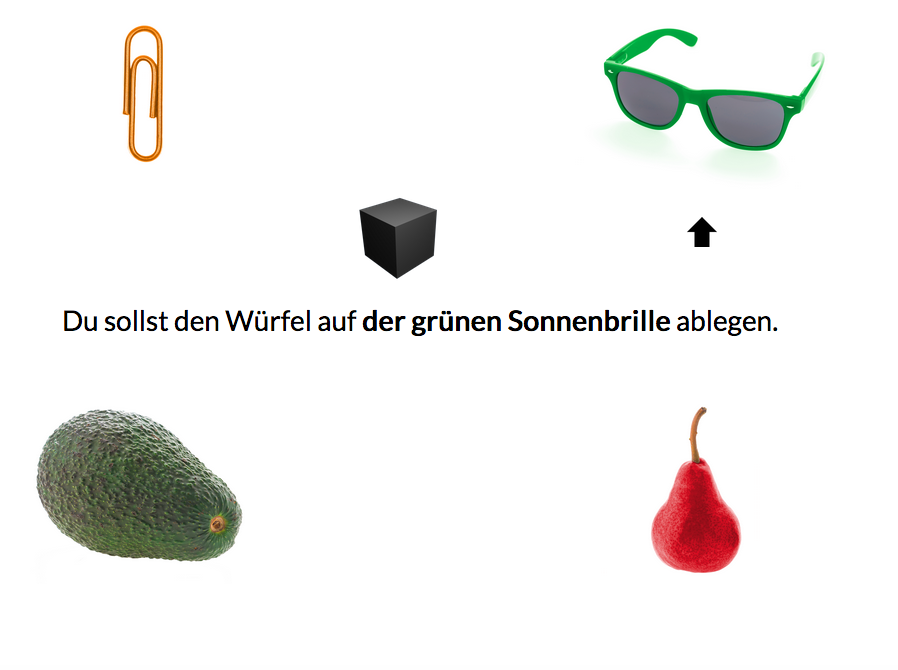
\includegraphics[width=0.6\linewidth,frame]{/Users/ste/repos/many_analyses/figs/sample_experiment_screen_competitor} 

}

\caption{Test trial: Example screen of a trigger instruction. The trigger instruction is displayed in the middle below the cube. Here, the participants have to instruct the experimenter to move the cube on top of the green sunglasses (indicated by an arrow).}\label{fig:image1}
\end{figure}

Each test trial consisted of two parts.
The trigger instruction and the test instruction.
After the preview of all images was displayed for 1500 ms, the competitor object was visually highlighted by an arrow, and a trigger instruction was presented in writing below the cube (see Figure \ref{fig:image1}).
The trigger instruction was constituted by the frame sentence \emph{Du sollst den Würfel auf X ablegen}.
\emph{X} was one of the adjective-noun combinations.

For example, the subjects saw the following sentence:

\ex \begingl
\glpreamble Du sollst den Würfel auf der grünen Sonnenbrille ablegen.//
\gla du sollst den würfel auf der grünen sonnenbrille ablegen.//
\glb you have.to the cube on the green sunglasses put//
\glft `You have to put the cube on top of the green sunglasses.'//
\endgl \xe

The trigger instruction was supposed to create a discourse context, such that both the color and the competitor object were introduced as background information into the discourse (in this example: \emph{green} and \emph{sunglasses}).
The trial proceeded when the experimenter has moved the cube onto the respective referent, at which point the sentence and the arrow would disappear.

Subsequently, the target object was visually highlighted by an arrow and the test instruction containing the target object was presented (see Figure \ref{fig:image2}).
This time the frame sentence was \emph{Und jetzt sollst du den Würfel auf X ablegen}, where \emph{X} was again an adjective-noun combination.
To continue the example above, the subject would see the following test instruction:

\ex \begingl
\glpreamble Und jetzt sollst du den Würfel auf der grünen Avokado ablegen.//
\gla und jetzt sollst du den würfel auf der grünen avokado ablegen//
\glb and now have.to you the cube on the green avocado put//
\glft `And now, you have to put the cube on top of the green avocado.'//
\endgl \xe

\begin{figure}[tbp]

{\centering 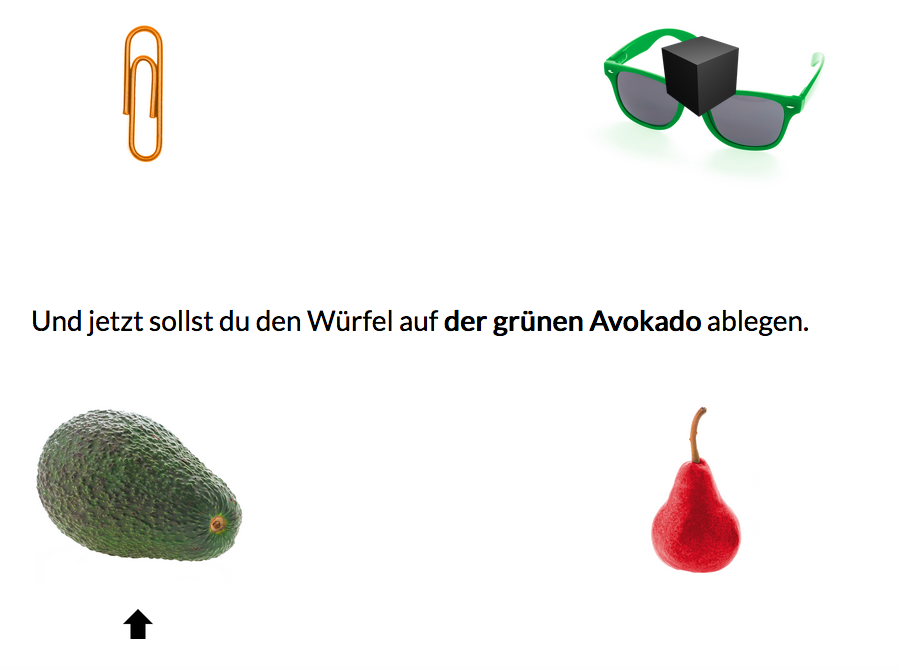
\includegraphics[width=0.6\linewidth,frame]{/Users/ste/repos/many_analyses/figs/sample_experiment_screen_target} 

}

\caption{Test trial: Example screen of the test instruction. The target sentence is displayed in the middle of the screen. Now, participants have to instruct the experimenter to move the cube on top of the green avocado (indicated by an arrow).}\label{fig:image2}
\end{figure}

The trial was completed and the next trial initiated as soon as the experimenter had moved the cube to the target referent.
There was a 3000 ms inter stimulus interval between trials (grey screen).
In both competitor and target sub sequences, the arrow was displayed with a lag of 1000 ms and the target sentence with a lag of 1500 ms in order to give participants sufficient time to glance at all referents before they were able to identify the relevant object and the instructions.

Using the trigger instruction to set up the discourse context enabled us to manipulate the focus structure of the target sentence.
If the color of the competitor and the target are of the same object type but differed in color (e.g.~\emph{yellow banana} vs \emph{blue banana}), the color adjective was discourse-pragmatically focused (henceforth the Adjective Focus (AF) condition).
If the objects differed but their color did not (e.g.~\emph{yellow banana} vs \emph{yellow tomato}), the noun was in focus (henceforth the Noun Focus (NF) condition).
If both the color and the object differed (e.g.~\emph{yellow banana} vs \emph{blue tomato}), the whole noun phrase was in focus (henceforth the Adjective/Noun Focus (ANF) condition).

There were 15 NF trials, 10 AF and 10 ANF trials each.
Each trial occurred two times per participants, yielding a total of 70 trials per participant.

The program (implemented as a browser-based application) used for the experiment is available at the following link: \url{https://github.com/SBRitter/fruits-production}.

\appendix

\hypertarget{random}{%
\section{Randomization}\label{random}}

In the production study, the combination of target/competitor/distractors were randomized in each trial.
Randomization was restricted to satisfy the following criteria, depending on the condition.

\begin{itemize}
\tightlist
\item
  NF-Condition:

  \begin{itemize}
  \tightlist
  \item
    Color of Target = Color of Competitor.
  \item
    Object of Target != Object of Competitor.
  \end{itemize}
\item
  AF-Condition:

  \begin{itemize}
  \tightlist
  \item
    Color of Target != Color of Competitor.
  \item
    Object of Target = Object of Competitor.
  \end{itemize}
\item
  DF-Condition:

  \begin{itemize}
  \tightlist
  \item
    Color of Target != Color of Competitor.
  \item
    Object of Target != Object of Competitor.
  \end{itemize}
\item
  Distractors, all conditions:

  \begin{itemize}
  \tightlist
  \item
    Both distractors have to differ in color and object identity from both target and competitor.
  \end{itemize}
\end{itemize}

The competitor and distractors were matched iteratively to a target.
One competitor could only be used twice or a third time if all other competitors that were left had been considered and proved inappropriate.

The set of four objects (quadruple) was formed separately for each of the three focus conditions.
After the three lists had been compiled, they were merged.
The sequence of quadruples was randomized such that the following requirements were met:

\begin{itemize}
\tightlist
\item
  The target color of one quadruple must not be equal to the competitor color of the following quadruple in order to avoid a contrastive focus on the next competitor noun.
\item
  The target object of one quadruple must not be equal to the competitor object of the following quadruple to avoid a contrastive focus on the next competitor adjective.
\item
  The list can have the same experimental condition in adjacent trials only in maximally 12\% of all cases.
\end{itemize}

Following these criteria, one randomized list for each subject was produced.
The list was then copied and merged with the first list in order to ensure that each unique trial occurs twice during one recording session.
In case the copy-and-merge procedure led to violation of any of the criteria described above, the first trial of the repetition list was shuffled until the criteria were met.

The python code for the randomization is available at the following link: \url{https://github.com/SBRitter/fruits-randomization}.

\end{document}
